\documentclass[12pt, titlepage, a4paper]{article}
\usepackage[utf8]{inputenc}
\usepackage{changepage}
\usepackage{prftree}
\usepackage{amssymb}
\usepackage{amsmath}
\usepackage{enumitem} 
\usepackage{graphicx}
\usepackage{wrapfig}
\usepackage[spanish]{babel}
\usepackage{amsthm}
\usepackage{bussproofs}
\usepackage{bm}
\usepackage{url}
\usepackage{hyperref}
\usepackage{dirtytalk}

\usepackage[edges]{forest}
\definecolor{folderbg}{RGB}{165, 105, 189}
\definecolor{folderborder}{RGB}{165, 105, 189}
\newlength\Size
\setlength\Size{4pt}
\tikzset{%
  folder/.pic={%
    \filldraw [draw=folderborder, top color=folderbg!50, bottom color=folderbg] (-1.05*\Size,0.2\Size+5pt) rectangle ++(.75*\Size,-0.2\Size-5pt);
    \filldraw [draw=folderborder, top color=folderbg!50, bottom color=folderbg] (-1.15*\Size,-\Size) rectangle (1.15*\Size,\Size);
  },
  file/.pic={%
    \filldraw [draw=folderborder, top color=folderbg!5, bottom color=folderbg!10] (-\Size,.4*\Size+5pt) coordinate (a) |- (\Size,-1.2*\Size) coordinate (b) -- ++(0,1.6*\Size) coordinate (c) -- ++(-5pt,5pt) coordinate (d) -- cycle (d) |- (c) ;
  },
}
\forestset{%
  declare autowrapped toks={pic me}{},
  pic dir tree/.style={%
    for tree={%
      folder,
      font=\ttfamily,
      grow'=0,
    },
    before typesetting nodes={%
      for tree={%
        edge label+/.option={pic me},
      },
    },
  },
  pic me set/.code n args=2{%
    \forestset{%
      #1/.style={%
        inner xsep=2\Size,
        pic me={pic {#2}},
      }
    }
  },
  pic me set={directory}{folder},
  pic me set={file}{file},
}

\usepackage{listings}

\usepackage{blindtext}
\usepackage[a4paper, total={6in, 8in}]{geometry}

\title{Trabajo Practico Final \\ 
Análisis del Lenguaje de Programación \\
Sistema F}
\author{Ramiro Gatto}
\date{21/04/2025}

\begin{document}
\maketitle

\section{Descripción del Proyecto}
La idea principal del proyecto es la de implementar un EDSL sobre el Sistema F, el cual permita la evaluación de algunos términos del mismo. Para  
que el proyecto sea simple se eligieron un par de tipos bases para el evaluador, los cuales son: 
\begin{itemize}[label=$\bullet$]
    \item {Empty}
    \item {Booleanos}
    \item {Naturales}
    \item {Funciones}
    \item {Listas (de cualquier tipo)}
\end{itemize}

\noindent Además, para el evaluador también se definió lo siguiente:
\begin{itemize}[label=$\bullet$]
    \item {Chequeador de tipos.}
    \item {Pretty-printer.}
    \item {Parser.}
\end{itemize}

Para poder realizar el mismo se tomo como inspiración el Trabajo Practico Nº2 \cite{tp2:lambdaCalculoSimpleTipado}, el cual se 
extendió/modifico para satisfacer con lo requerido.


\section{Manual de uso e Instalación del software}
Para poder usar el evaluador se va a necesita de Stack \cite{haskellStack}, una vez instalado se tiene que abrir una consola en el 
directorio del proyecto (Sistema-F) y ejecutar:
\begin{enumerate}
    \item stack setup (una única vez)
    \item stack build
    \item stack exec Sistema-F-exe
\end{enumerate}

\noindent Con las dos primeras lineas compilamos el proyecto y con la tercera lo ejecutamos.


\section{Organización de los archivos}
\noindent La organización de los archivos del proyecto es la siguiente:

\begin{forest}
    pic dir tree,
    where level=0{}{
      directory,
    },
  [Sistema-F
    [.stack-work]
    [app
     [Main.hs, file]
    ]
    [dist-newstyle]
    [src
     [Common.hs, file]
     [Parse.y, file]
     [PrettyPrinter.hs, file]
     [SystemF.hs, file]
    ]
    [.gitignore, file]
    [CHANGELOG.md, file]
    [Ejemplos.txt, file]
    [LICENSE, file]
    [package.yaml, file]
    [README.md, file]
    [Sistema-F.cabal, file]
    [stack.yaml, file]
    [stack.yaml.lock, file]
  ]
\end{forest}

Para entender como funciona el proyecto veamos la función de los archivos en las carpetas app y src que son los principales para 
el funcionamiento del mismo, el resto de los archivos son de configuración.

\subsection{app}
\subsubsection{Main.hs}
Este archivo es donde comienza la ejecución del programa al compilarse y ejecutarse. Hace uso de una 
serie de funciones para poder parser la entrada por teclado, determinar el comando ingresado, 
imprimir por pantalla, realizar la evaluación, entre muchas cosas más.\\

Parte del \textbf{Main.hs} es idéntico al del TP Nº2 \cite{tp2:lambdaCalculoSimpleTipado}, excepto por algunas modificaciones y simplificaciones para que 
se ajuste al comportamiento requerido.

\subsection{src}
\subsubsection{Common.hs}
En este archivo es donde se definen la forma que tendrán los valores, términos y tipos del Sistema F. Para estos nos basamos en la gramática del mismo.

\subsubsection{Parse.y}
Para generar el parser utilizaremos happy. En este archivo se generan los parsers a utilizar, se definen los tokens que acepta el parse, 
entre más funciones. También es donde se define el lexer que se utilizara como analizador lexicográfico de la entrada. \\ 

Se tiene 2 parses, uno es el parseStmt en donde el no terminal de nivel superior (top-level non-terminal) es \textbf{Def} y el 
segundo en donde el top-level non-terminal es \textbf{Exp}. 
Para crear el archivo se utilizo parte del Parser.y del TPº2 \cite{tp2:lambdaCalculoSimpleTipado} y la documentación de Happy \cite{haskellHappy}. \\

\subsubsection{PrettyPrinter.hs}
Para poder mostrar los términos se utilizo la biblioteca pretty printing, la cual consiste en una serie de combinados desarrollada por John Hughes. Aca es 
donde se encuentra implementado el pretty printer para el Sistema F. \\
En este podemos distinguir 2 función importantes:
\begin{itemize}[label=$\bullet$]
  \item {\textbf{printType}: la cual se encarga de imprimir por pantalla los Type.}
  \item {\textbf{printTerm}: la cual dado un Term lo imprime por pantalla.}
\end{itemize}

\subsubsection{SystemF.hs}
En este archivo es donde se implementan las funciones de evaluación y el chequeador de tipo (además de unas cuantas funciones auxiliares 
para el correcto funcionamiento).

\section{Decisiones de diseño importantes}
\subsection{Representación del Sistema F}
Los tipos, términos y valores en el Sistema F están dados por la siguientes gramática, respectivamente:
\begin{align*}
    T &::= E \mid T \rightarrow T \mid X \mid \forall X \ . \ T \mid Bool \mid Nat \mid List \ T\\
    t &::= x \mid \lambda x:T. \ t \mid t \ t \mid ifthenelse \ t \ t \ t \mid True \mid False \mid 0 \mid suc \ t \mid  nil \mid  \\
    & \ \ \ \ \ \ cons \ t \ t \mid R \ t \ t \ t \mid RL \ t \ t \ t \mid \Lambda X \ . \ t \mid t \ \langle X \rangle \\
    v &::= True \mid False \mid nv \mid lv \mid \lambda x:T. \ t \mid \Lambda X \ . \ t \\
    nv &:: = 0 \mid suc \ nv \\
    lv &:: = nil \mid cons \ v \ lv \\
\end{align*}

Como se menciono anteriormente, la implementación de estos se encuentra en el archivo \textbf{src/Common.hs} y es la siguiente:

\noindent Para los tipos es:
\begin{verbatim}
    data Type = EmptyT 
              | FunT Type Type
              | BoundForAll Pos
              | VarT String
              | ForAllT Fat
              | BoolT
              | NatT
              | ListTEmpty
              | ListT Type
              deriving (Show, Eq)

    data Pos = External Int | Inner Int deriving (Show)
    instance Eq Pos where
        External t1 == Inner t2    = t1 == t2
        Inner t1    == External t2 = t1 == t2
        External t1 == External t2 = t1 == t2
        Inner t1    == Inner t2    = t1 == t2
    
    data Fat = Lambd Type | Lt String Type | Ty Type deriving (Show)
    instance Eq Fat where
        Ty  t1   == Lambd t2 = t1 == t2
        Lambd t1 == Ty  t2   = t1 == t2
        Lt _ t1  == Lambd t2 = t1 == t2
        Lambd t1 == Lt _ t2  = t1 == t2
        Ty t1    == Lt _ t2  = t1 == t2
        Lt _ t1  == Ty t2    = t1 == t2
    
        Lt s t1  == Lt s' t2 = t1 == t2 && s == s'   
        Ty t1    == Ty t2    = t1 == t2
        Lambd t1 == Lambd t2 = t1 == t2
\end{verbatim}

De esta definición se pueden ver muchas cosas, asi que vayamos por parte. Empecemos con la declaración del Type, esta se basa en la gramática del Sistema F, pero 
posee \say{2 elementos} de más, los cuales son: 

\begin{itemize}[label=$\bullet$]
  \item {\textbf{ListTEmpty}\\
  Como se van a poder usar listas de todo tipo surge un problema a la hora de usar una lista vacía, ya que se debería especificar el tipo, 
  a pesar de estar vacía. 
  Para evitar complicaciones y simplificar esto, lo que decidí fue darle un tipo especial a la lista vacía, \textbf{ListTEmpty}, de esta forma se evita 
  tener que darle un tipo especifico.
  
  Teniéndose que agregar un caso \say{especial} para lista vacía en las funciones que pueden recibir una como argumento (como infer' o match)
  }

  \item {\textbf{BoundForAll}\\
  En este caso, este no es un tipo per se, sino que su función es similar a la idea 
  de los indices de De Brujin. Esto seria, coloquialmente hablando, indicar a que \textbf{para todo} esta ligada la variable cuantificada, 
  en un inicio la idea fue la siguiente:

  \begin{center}
      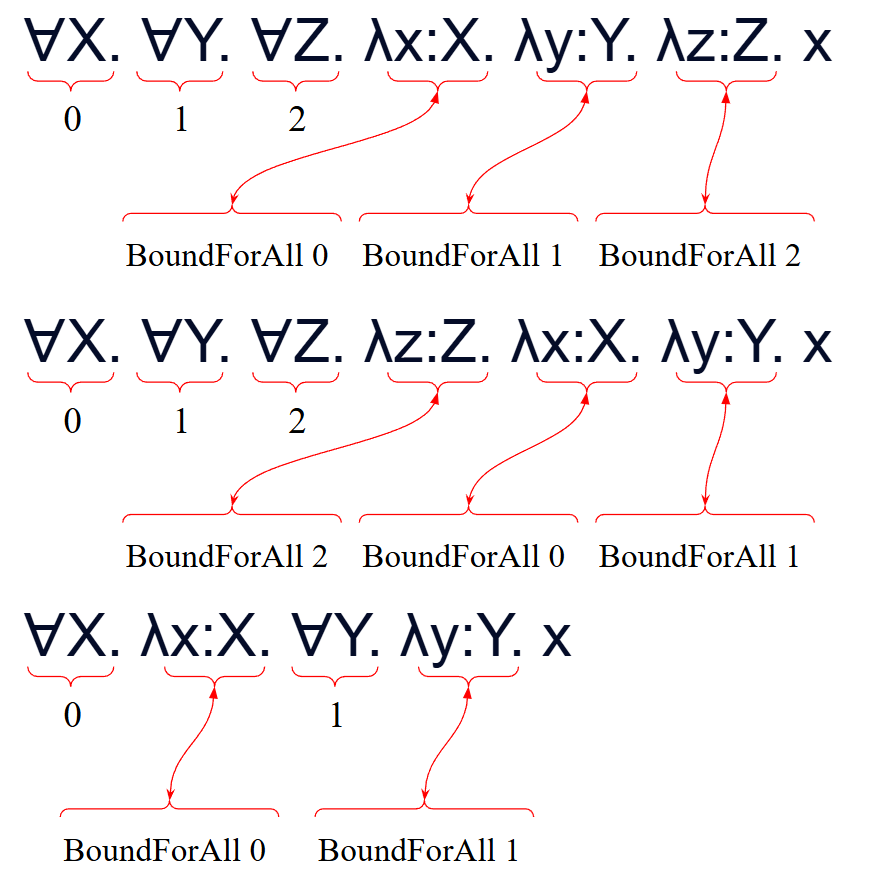
\includegraphics[width=0.7\textwidth]{Imagenes/EjemploBoundForAll.png}
  \end{center}

  Es decir, que solo se almacene el \textbf{para todo} al cual esta ligado. 
  Al principio la idea era poner (BoundForAll Int) con los Term (como el Bound que esta en Term), pero como esta idea esta relacionada con 
  los tipos resulto más practico agregarlo aca.\\
  
  Pero a medida que se fue avanzando con el Proyecto la idea de usar solo algo de la forma (BoundForAll Int) resulto insuficiente, ya que podría ocurrir algo 
  como en el siguiente ejemplo:
  
  \begin{center}
    %(/\textbackslash A. \textbackslash a:A. \textbackslash b:(\textbackslash/B. \textbackslash/A. A -$>$ B) . b) 
    $\Lambda$A. $\lambda$a:A. $\lambda$b: ($\forall$B. $\forall$A. A $\rightarrow$ B)
  \end{center}

  Si solo se usa la forma (BoundForAll Int) estos se pondrían en los siguientes lugares:

  \begin{center}
    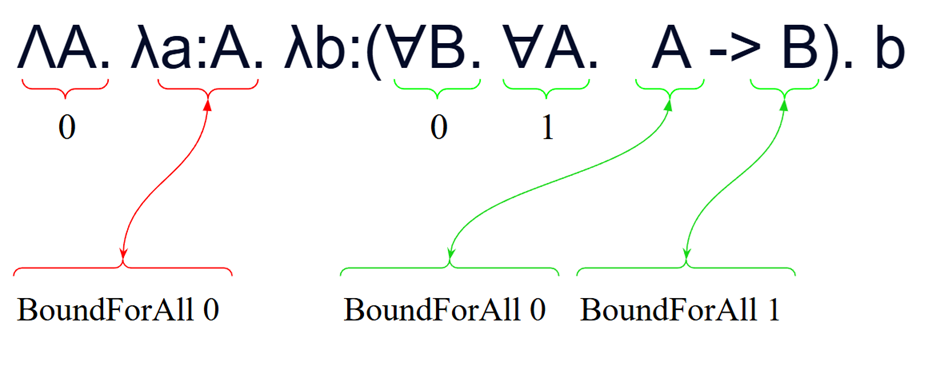
\includegraphics[width=.8\textwidth]{Imagenes/EjemploBoundForAllFunction.png}
  \end{center}

  Donde se puede apreciar que se tiene un solo $\Lambda$ pero tenemos (BoundForAll 0) y (BoundForAll 1). Uno tendería a 
  pensar que esto es un error, pero no lo es ya que estos BoundForAll no están \say{ligados} al $\Lambda$ sino al $\forall$.\\

  Debido a esto surge la necesidad de poder distinguir cuando un BoundForAll esta \say{dentro} o \say{afuera}. 
  Entonces para indicar a cual esta ligado un a variable se introduce el tipo Pos, donde External y Inner indican a que $\Lambda$ y a que $\forall$ esta 
  ligado respectivamente. 
  Una cuestión es que los External son \say{globales} y los Inner \say{locales}, usemos este ejemplo para ilustrar esto:


  \begin{center}
    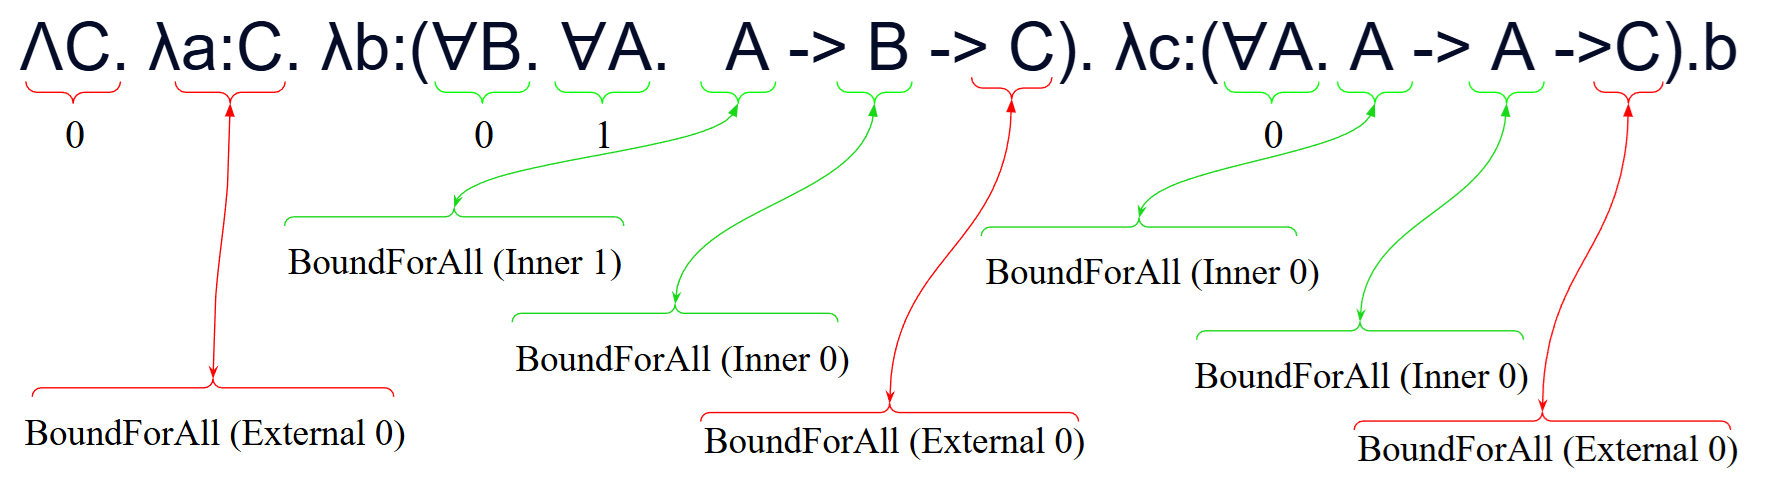
\includegraphics[width=1\textwidth]{Imagenes/EjemploBoundForAllFunction3.png}
  \end{center}

  En donde el Int que posee el External de $\Lambda$C. se respeta en todos lados, mientras que el $\forall$A. se tiene en b con (Inner 1) y en c con (Inner 0). 
  Es decir, el Inner depende del tipo actual, mientras que el External es el mismo sin importar donde este.

  Además, hay que tener en cuenta una cosa más, los dos tipos de Pos deben ser iguales entre si, para que se pueda hacer este tipo 
  de sustitución.
  
  \begin{center}
    ($\lambda$x: ($\forall$Y. Y $\rightarrow$ Y). x) ($\Lambda$X. $\lambda$x:X. x)
  \end{center} 

  Ya que en la primera el tipo de x seria algo del estilo,
  \begin{center}
    (BoundForAll (Inner 0)) $\rightarrow$ (BoundForAll (Inner 0)). 
  \end{center}
  Mientras que en la segunda expresión seria de tipo 
  \begin{center}
    (BoundForAll (External 0)) $\rightarrow$ (BoundForAll (External 0)). 
  \end{center}
  
  Por lo que la única forma de poder hacer la sustitución es que Externa e Inner sean iguales (Esto 
  se logra definiendo mi propio Eq de Pos). \\

  Otra razón para distinguir entre Inner y External es cuando se realize una aplicación de la forma,
  \begin{center}
    $\Lambda$X. t $<$TipoNuevo$>$
  \end{center} 
   asi al reemplazar se reemplazaría los BoundForAll (External k) y no los Inner (lo cual estaría mal).
  }
  \end{itemize}

  Una decision de diseño importante fue el \textbf{ForAllT Fat}, en un inicio la idea del tipo \textbf{Fat} era tener solo 2 
  constructores los cuales eran el \textbf{Lambd Type} y el \textbf{Ty Type}, los cuales servían para distinguir el 
  \say{$\Lambda$} y el \say{$\forall$} en las expresiones a la hora de imprimir por pantalla. \textbf{Lambd} aparece solo cuando se quiere ver el tipo de 
  la expresión, \textbf{Ty} se utiliza en el tipo de las variables 
  (es decir, siempre va a estar en la expresión). Si no se hiciese la distinción entre \textbf{Lambd} y  \textbf{Ty}, al querer imprimir tipos como:

  \begin{center}
    ($\Lambda$A. $\lambda$a:A. $\lambda$b:($\forall$B. B -$>$ B). b)
  \end{center}  
  se producirían incongruencias, ya que no se puede distingue entre \say{$\Lambda$} y el \say{$\forall$}. Al agregar el tipo \textbf{Fat} se puede 
  hacer esta distinción  y se evita el problema.\\

  Todavía hay un problema importante con los tipo si al \textbf{Fat} se lo deja solo con esos 2 constructores, hay problemas al momento de parsear 
  expresiones como,

  \begin{center}
    ($\lambda$x:($\forall$X. $\forall$Y. $\forall$Z. X -$>$ Z -$>$ Z). x)
  \end{center}  
  es decir, el tipo posee más $\forall$ de los que se utiliza, y es dificl de determinar a $\forall$ estan ligados las variables. 
  Para solucionarlo se agrega el tipo \textbf{Lt String Type}. \\
  
  Lo que se hace es que 
  al momento de parsear la expresión entrante se utiliza el \textbf{Lt} para los $\forall$ de los tipos (y asi saber el nombre del $\forall$
  correspondiente), y luego cuando se hace la conversion de 
  LamTerm a Term, se realiza el reemplazo por \textbf{Ty}, evitando tener que almacenar devuelta el string.\\


\noindent Para las expresiones del lambda calculo se tiene:
\begin{verbatim}
    data LamTerm = LVar String
                 | LAbs String Type LamTerm
                 | LApp LamTerm LamTerm
                 | LTAbs String LamTerm
                 | LTApp LamTerm Type
                 | LTrue 
                 | LFalse
                 | LIfThenElse LamTerm LamTerm LamTerm
                 | LZero
                 | LSuc LamTerm
                 | LRec LamTerm LamTerm LamTerm
                 | LNil
                 | LCons LamTerm LamTerm
                 | LRecL LamTerm LamTerm LamTerm
                 deriving (Show, Eq)
\end{verbatim}

Al igual que en el Trabajo Practico 2 \cite{tp2:lambdaCalculoSimpleTipado} surge el problema del uso de nombre de variables, al 
momento de realizar operaciones como la sustitución. Para arreglar esto se mantiene la misma idea de 
usar la representación con \textbf{indices de De Brujin}. \\

Al usar una representación sin nombre surge el problema de no tener variables libres,  
para evitar este inconveniente se utiliza la representación localmente sin nombres (donde variables libres y ligadas están 
en diferentes categorías sintácticas). \\
\noindent Al utilizar esta representación los términos quedan asi:
\begin{verbatim}
    data Term = Bound Int
              | FreeGlobal String 
              | App Term Term
              | Lam Type Term
              | ForAll Term
              | TApp Term Type
              | T
              | F
              | IfThenElse Term Term Term
              | Zero
              | Suc Term
              | Rec Term Term Term
              | Nil
              | Cons Term Term
              | RecL Term Term Term
              deriving (Show, Eq)
\end{verbatim}

\noindent Una diferencia respecto al TP Nº2 \cite{tp2:lambdaCalculoSimpleTipado} es que se elimino el tipo,
\begin{verbatim}
  data Name = Global String deriving (Show, Eq)  
\end{verbatim}
y en su lugar, ahora, solo se utiliza String. Esta decision se debe a que en el archivo \textbf{Main.hs} originalmente se usaba la función 
nub para el comando \textbf{:browse}, teniendo esta un costo de O($n^2$). Al realizar este reemplazo fue posible definir mi propio nub 
con costo O($n\cdot lg(n)$). \\

En el único lugar que se usaba \say{Name} en Trabajo Practico 2 era en el constructor \say{Free} (en Term), 
entonces para no perder la idea de que \say{Name} se usaba para 
representar nombres de variables \say{globales libres} (Free (Global String)), lo que se hizo fue cambiar el constructor \say{Free Name} por 
\say{FreeGlobal String} y mantener esa idea. 

\subsubsection{Evaluación}
Para la evaluación el interprete sigue el orden de reducción \textbf{call-by-value} en donde tenemos las siguientes reglas, las cuales 
son las presentes en el TP Nº2 \cite{tp2:lambdaCalculoSimpleTipado} y en el material de clase del Sistema F \cite{ALP:Polimorfismo}:

\begin{displaymath}
    \prftree[r]{(E-App1)}{t_1 \rightarrow t_1'}{t_1 \ t_2 \rightarrow t_1' \ t_2}  \hspace{1cm}
    \prftree[r]{(E-App2)}{t_2 \rightarrow t_2'}{v \ t_2 \rightarrow v \ t_2'}  \hspace{1cm}
    \prftree[r]{(E-AppAbs)}{}{(\lambda x : T_1 \ . \ t_1 ) v \rightarrow t_1[x/v]}
\end{displaymath}

\begin{displaymath}
    \prftree[r]{E-IFTrue}{ifthenelse \ T \ t_2 \ t_3}{t_2} \hspace{0.5cm}
    \prftree[r]{E-IFFalse}{ifthenelse \ F \ t_2 \ t_3}{t_3} \hspace{0.5cm}
\end{displaymath}
\begin{displaymath}
    \prftree[r]{E-IF}{t_1 \rightarrow t_1'}{ifthenelse \ t_1 \ t_2 \ t_3 \rightarrow ifthenelse \ t_1' \ t_2 \ t_3}
\end{displaymath}

\begin{displaymath}
    \prftree[r]{E-RZero}{R \ t_1 \ t_2 \ 0 \rightarrow t_1} \hspace{0.5cm}
    \prftree[r]{E-RSuc}{R \ t_1 \ t_2 (suc \ t) \rightarrow t_2 (R \ t_1 \ t_2 \ t) t} \hspace{0.5cm}
    \prftree[r]{E-R}{t_3 \rightarrow t_3'}{R \ t_1 \ t_2 \ t_3 \rightarrow R \ t_1 \ t_2 \ t_3'}
\end{displaymath}


\begin{displaymath}
    \prftree[r]{E-RNil}{RL \ t_1 \ t_2 \ nil \rightarrow t_1} \hspace{0.5cm}
    \prftree[r]{E-RCons}{RL \ t_1 \ t_2 (cons \ t \ l) \rightarrow t_2 \ t \ l \ (RL \ t_1 \ t_2 \ l)} \hspace{0.5cm}
\end{displaymath}
\begin{displaymath}
    \prftree[r]{E-RL}{t_3 \rightarrow t_3'}{RL \ t_1 \ t_2 \ t_3 \rightarrow RL \ t_1 \ t_2 \ t_3'} \hspace{0.5cm}
\end{displaymath}
\begin{displaymath}
  \prftree[r]{E-Cons1}{t_1 \rightarrow t_1'}{cons \ t_1 \ t_2 \rightarrow cons \ t_1' \ t_2} \hspace{0.5cm}
  \prftree[r]{E-Cons2}{t_2 \rightarrow t_2'}{cons \ t_1 \ t_2 \rightarrow cons \ t_1 \ t_2'} \hspace{0.5cm}
\end{displaymath}


\begin{displaymath}
    \prftree[r]{E-TApp}{t_1 \rightarrow t_1'}{t_1 \ \langle T \rangle \rightarrow t_1' \ \langle T \rangle} \hspace{1cm}
    \prftree[r]{E-TAppAbs}{(\Lambda X \ . \ t)\ \langle T \rangle \rightarrow t[X/T]}
\end{displaymath}

\subsubsection{Tipos}
Para realizar la inferencia de tipo usamos las siguientes reglas, las cuales al igual que en la sección anterior son las
presentes en el TP Nº2 \cite{tp2:lambdaCalculoSimpleTipado} y en el material de clase del Sistema F \cite{ALP:Polimorfismo}:

\begin{displaymath}
    \prftree[r]{T-True}{\Gamma \vdash T: Bool} \hspace{0.5cm}
    \prftree[r]{T-False}{\Gamma \vdash F:  Bool} \hspace{0.5cm}  
    \prftree[r]{T-IF}{\Gamma \vdash t_1 : Bool}{\Gamma \vdash t_2 : T}{\Gamma \vdash t_3 : T}{\Gamma \vdash ifthenelse \ t_1 \ t_2 \ t_3 \ : \ T} \hspace{1cm}
\end{displaymath}

\begin{displaymath}
    \prftree[r]{T-Zero}{\Gamma \vdash 0 : Nat} \hspace{1cm}
    \prftree[r]{T-Suc}{\Gamma \vdash t : Nat}{\Gamma \vdash suc \ t : Nat} \hspace{1cm}
\end{displaymath}
\begin{displaymath}
    \prftree[r]{T-Rec}{\Gamma \vdash t_1 : T}{\Gamma \vdash t_2 : T \ \rightarrow \ Nat \rightarrow \ T}{\Gamma \vdash t_3 : Nat}{\Gamma \vdash R \ t_1 \ t_2 \ t_3 : T} \hspace{1cm}
\end{displaymath}

\begin{displaymath}
    \prftree[r]{T-Nil}{\Gamma \vdash nil : ListEmpty} \hspace{1cm}
    \prftree[r]{T-Cons}{\Gamma \vdash t_1 : T}{\Gamma \vdash t_2 : List \ T}{\Gamma \vdash cons \ t_1 \ t_2 :  List \ T} \hspace{1cm}
\end{displaymath}
\begin{displaymath}
    \prftree[r]{T-RL}{\Gamma \vdash t_1 : T}{\Gamma \vdash t_2 : T_1 \ \rightarrow \ List \ T_1 \rightarrow \ T \rightarrow \ T}{\Gamma \vdash t_3 : List \ T_1}{\Gamma \vdash \ RL \ t_1 \ t_2 \ t_3 \ : \ T} \hspace{1cm}
\end{displaymath}

\begin{displaymath}
    \prftree[r]{T-TAbs}{\Gamma, X \vdash t : T}{\Gamma \vdash \Lambda X \ . \ t : \forall X \ . \ T} \hspace{1cm}
    \prftree[r]{T-TApp}{\Gamma \vdash t_1 : \forall X \ . \ T}{\Gamma \vdash t_1 \langle T_2 \rangle : T[X/T_2]} \hspace{1cm}
\end{displaymath}

\subsection{Mostrar términos}
Al igual que en el TP Nº2 \cite{tp2:lambdaCalculoSimpleTipado} se va a utilizar la biblioteca \textbf{pretty printing} para mostrar por 
pantalla. En el archivo
\textbf{src/PrettyPrinter.hs} es donde se implementa el \textbf{pretty printing} para el sistema F.

\subsection{Ejemplos con resultados}
Una vez que se haya compilado y ejecutado el programa nos aparecerá en la consola esto:

\begin{verbatim}
Intérprete de Sistema F
Escriba :help para recibir ayuda.
SF>
\end{verbatim}

Luego si se quiere evaluar una expresión del Sistema F, se la ingresa por teclado, se presiona el enter y listo 
(también hay más opciones como el :print para mostrar los ASTs y el :type para ver el tipo de la expresión, entre muchas otras). \\

Una libertad que me tome al momento de mostrar por pantalla es 
en el tema de los Bool, que si bien en la gramática el if aparece como \textbf{ifthenelse $t_1$ $t_2$ $t_3$} y 
tanto en los LamTerm como en los Term también aparece con esta forma, a la hora de escribirlo y mostrarlo por consola es 
\textbf{if $t_1$ then $t_2$ else $t_3$}, este cambio se hizo por comodidad y para que sea más legible, es más común escribirlo como la segunda forma que como 
la primera.\\

Otra libertad fue con los Naturales, lo que se hace es evitar mostrar el \textbf{suc} todas las veces que aparece, sino que se usa 
la forma de \textbf{suc$^x$} (donde x representa la cantidad de veces que aparece el \textbf{suc} en el Natural). \\

Veamos ejemplos (estos ejemplos están en el archivo Ejemplos.txt para que puedan ser testeados sin problemas por el lector):

\subsubsection{Funcion identidad polimorfica}
\noindent En el Sistema F se escribiría: $\Lambda X.\ \lambda $x:X$. \ x$ \\
En la consola escribimos: /\textbackslash X. \textbackslash x:X . x \\
Si quisiéramos evaluarla a un natural escribimos: (/\textbackslash X. \textbackslash x:X . x)  $<$Nat$>$ (suc 0) \\
El cual se reduce a: suc 0

\subsubsection{Funcion length para listas polimorfica}
\noindent En el Sistema F se escribiría: $\Lambda X.\ \lambda xs:List \ X. \ $RL 0 $(\lambda $x:X$ \ .$ys:List X$ \ .$r:Nat$\ .suc\ r)\ xs$ \\
En la consola escribimos: (/\textbackslash X. (\textbackslash xs:List X. RL 0 (\textbackslash x:X .\textbackslash ys:List X. \textbackslash r:Nat. suc r) xs)) \\
Si quisiéramos evaluarla a una lista de funciones polimorficas escribimos: 
((/\textbackslash X. (\textbackslash xs:List X. RL 0 (\textbackslash x:X .\textbackslash ys:List X. \textbackslash r:Nat. suc r) xs)) $<$\textbackslash/X. X -$>$ X$>$) 
(cons (/\textbackslash X. \textbackslash x:X. x) cons (/\textbackslash X. \textbackslash x:X. x) nil)\\
El cual se reduce a: suc$^2$ 0 \\

\noindent (Si se prueba con nil da como resultado 0)

\subsubsection{Funcion que toma como argumento una funcion polimorfica}
\noindent En el Sistema F se escribiría: $\Lambda A.\ \lambda a:A.\ \lambda b:(\forall B. B \rightarrow  B). \ b$ \\
En la consola escribimos: (/\textbackslash A. \textbackslash a:A. \textbackslash b:(\textbackslash /B. B -$>$ B) . b)\\
Si quisiéramos evaluarla podría ser algo asi: (/\textbackslash A. \textbackslash a:A. \textbackslash b:(\textbackslash /B. B -$>$ B) . b) $<$Nat$>$ 0 (/\textbackslash X. \textbackslash x:X. x) $<$Bool$>$ T\\
El cual se reduce a: T

\section{Documentación Haddock (Bonus)}
Como algo adicional se pensó en usar Haddock \cite{HaddockDoc} para documentar las principales funciones de los módulos en src.
Para ver dicha documentación se puede usar el comando:
\begin{center}
  stack haddock --no-haddock-deps --open
\end{center}

\newpage

\bibliographystyle{unsrt}
\bibliography{lib}

\end{document}